% $Id: introduction.tex 34630 2013-04-29 22:53:51Z roldeman $

\section{The $\alpha_T$ analysis at CMS}
\label{sec:Introduction}

The Standard Model (SM) is the most successful scientific theory to date \cite{Salam1964}\cite{Glashow1961}\cite{Weinberg1967}. It makes accurate predictions about the physical world that have consistently stood up to experimental scrutiny. This culminated in the discovery of a $125$~GeV particle consistent with a Higgs boson at the Large Hadron Collider (LHC) in 2012~\cite{ATLASHiggs2012}\cite{CMS2012HiggsPaper}. Despite this, the SM is incomplete; neither including a description of gravity or dark energy, nor providing a suitable dark matter candidate.
\\\\
If there is to be a theory of everything, it is assumed new physics must be present at the Planck scale\footnote{Around $1.22\times 10^{19}$GeV}, where gravity becomes relevant. The mass of the Higgs receives quantum corrections from the virtual effects of every particle that couples to it. If new physics exists at the Planck scale it will have an overwhelmingly large contribution to the mass of the Higgs. As the Higgs exists at the electroweak scale, the quantum corrections must mostly cancel each other out. The only way to achieve this without new physics at the electroweak scale is with an incredible fine tuning of parameters, which is known as the ``hierarchy problem'' \cite{SUSYprimerMartin:1997ns}. 
\\\\
A natural cancellation of corrections to the Higgs mass can be provided by the introduction of a new broken spacetime symmetry between fermions and bosons known as Supersymmetry (SUSY). As fermions and bosons provide opposite sign corrections to the Higgs mass, the existence of SUSY close the electroweak scale solves the hierarchy problem. Additionally, in the case that R-parity\footnote{$R\equiv (-1)^{3(B-L)+2s}$, where $B$ is the baryon number, $L$ the lepton number and $s$ the spin.} is conserved, SUSY models can provide a candidate for Dark Matter in the form of a weakly interacting lightest supersymmetric particle (LSP). Another strong theoretical motivation for SUSY is the fact that it may also unify the strong, weak and electromagnetic forces at the GUT scale\footnote{The energy above which the strong, weak and electromagnetic forces are unified.}; this is not possible in the SM. The supersymmetric extension of the SM that introduces the fewest new particles exhibits the above features and is known as the Minimal Supersymmetric Standard Model (MSSM) \cite{SUSYprimerMartin:1997ns}.

% the alphaT bit

As motivated in Section~2, it is important to carry out a search for SUSY at the LHC in the hadronic jets plus missing transverse energy, $\cancel{E}_T$, final state. By considering only events with an all hadronic final state, vetoing isolated leptons, electroweak backgrounds can be suppressed. This is particularly important as the only genuine source of $\cancel{E}_T$ in the SM is neutrinos.
\subsection{Definition of \boldmath $\alpha_T$}
The major problem with purely hadronic events is the huge background from multijet events. QCD events can give fake $\cancel{E}_T$ signatures if one or more of the jets are mismeasured in the detector. To overcome this, the dimensionless variable $\alpha_T$ is introduced \cite{AlphaTproposalCMS:2008vya} \cite{AlphaTproposalPhysRevLett.101.221803}. For a dijet system it is defined as:
\begin{equation}
\alpha_T=\frac{E_T^{j_2}}{M_T},
\end{equation}
where $E_T^{j_2}$ is the energy of the lowest energy jet, $M_T=\sqrt{H_T^2-\cancel{H}_T^2}$ is the invariant mass of the dijet system. It is constructed from the jet characterising variables:
\begin{equation}
H_T=\sum_{i=1}^{n_{jet}}E_T^{j_i}, 
\end{equation}
and
\begin{equation}
\cancel{H}_T=|\sum_{i=1}^{n_{jet}}\vec{p}_T^{j_i}|,
\end{equation}
with $n_{jet}$ jets, $j_i$, with transverse momentum $\vec{p}_T^{j_i}$ and transverse energy $E_T^{j_i}$. For events with more than two jets a pseudo dijet system is formed by combining jets. The system chosen is one that minimises $|\Delta H_T|$. This is the difference between the $E_T$ of each pseudo jet, where $E_T$ is the scalar sum of the transverse energies of all the jets in each pseudo jet. This leads to a generalised form of $\alpha_T$ \cite{AlphaT8TeVChatrchyan:2013lya}:
\begin{equation}
\alpha_T=\frac{1}{2}\times\frac{H_T-\Delta H_T}{\sqrt{H_T^2-\cancel{H}_T^2}}
\end{equation}
In the case that two well measured back to back jets are produced by a QCD process, assuming the mass of the jet constituents is much less than the total energy of the jet, $\alpha_T=0.5$. If one of these jets is mismeasured, resulting in fake $\cancel{E}_T$, then $\alpha_T<0.5$. However, if the two jets are recoiling from genuine $\cancel{E}_T$ then $\alpha_T>0.5$. A cut on $\alpha_T$ of around $0.55$ can remove almost all QCD background. The power of this variable to eliminate QCD background can be seen in Fig.~\ref{fig:alphaT}.
\begin{figure}
	\begin{center}
		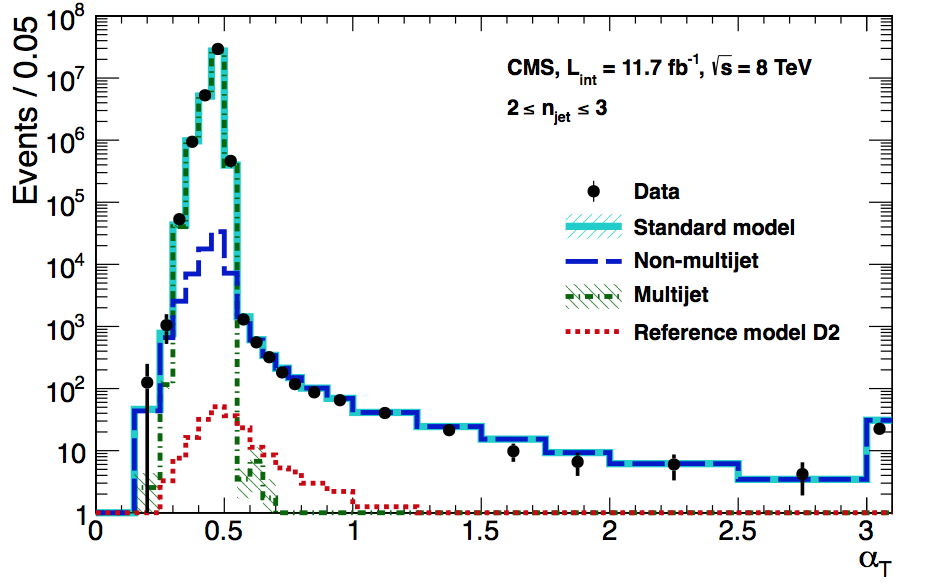
\includegraphics[width=0.8\linewidth]{alphaT1_bkgd}
	\end{center}
	\caption{The $\alpha_T$ values for events with $H_T>375$ GeV and 2 to 3 jets that pass all other cuts imposed in the $\alpha_T$ analysis. The green dotted line shows the expected multijet QCD background that can be removed with an appropriate cut on $\alpha_T$ \cite{AlphaT8TeVChatrchyan:2013lya}}
	\label{fig:alphaT}
\end{figure}
\subsection{The \boldmath $\alpha_T$ analysis}
Events are selected with at least one vertex with $p_T>50$~GeV jets, where the jets are well reconstructed in the central region, $|\eta|<3$. Events with isolated\footnote{A particle is isolated if there are no other particles within a cone of $\sqrt{(\Delta\phi)^2+(\Delta\eta)^2}=0.3$} leptons of $p_T>10$~GeV or photons of $p_T>25$~GeV are vetoed. Events are categorised based on the number of jets, the number of jets with a reconstructed b-quark and the value of $H_T$. This allows for a variable $\alpha_T$ cut based on the category, maximising signal acceptance. Full details of the analysis can be found at \cite{AlphaT8TeVChatrchyan:2013lya} and \cite{AlphaT_7TeV_PRLChatrchyan:2011zy}.

% the susy production bit

The LHC is a 27km circumference hadron synchrotron built on the Franco-Swiss border \cite{LHCMachine} near Geneva. It ran from 2010 to 2013 colliding protons at centre-of-mass energies $\sqrt{s}=7$ and $8$ TeV (Run 1), with detectors built around the beam collecting up to $23.3$~fb$^{-1}$ of data. Preparations are currently underway for Run 2 of the LHC at a full operating energy of $\sqrt{s}=13$ to $14$ TeV in 2015. This upgrade will have a maximum instantaneous luminosity of $1.6\times10^{34}$~cm$^{-2}$s$^{-1}$, more than twice the peak of $7.7\times10^{33}$~cm$^{-2}$s$^{-1}$ reached in 2012 \cite{LHCLuminosityIPAC13}. With this increase in energy and luminosity, potential for the discovery of new physics at the energy frontier is high.  
\\\\
\subsection{Supersymmetry production at the LHC}
As the LHC is a hadron collider, the highest cross section SUSY production processes occur via the strong force \cite{SUSYprimerMartin:1997ns} \cite{SUSYxsections_NewAspectsof_pp_collisions}. These processes result in the production of squarks and gluinos, the SUSY particles with colour charge. In all favoured SUSY models, these relatively heavy particles decay within the detector to a weakly interacting LSP, usually a neutralino \cite{SUSYPhe_hadronic_states_Farrar:1978xj}. In collisions at the LHC this will appear as several hard jets with unbalanced momentum (missing energy). 
\\\\
To interpret the results of SUSY searches simplified models are used. These models include a smaller number of SUSY particles than the MSSM, but allow the representation of event topologies in a consistent way \cite{SimplifiedModelsAlves:2011wf} \cite{MathiasSUSYthesis}. A simplified model representation of hadronic SUSY production and decay can be seen in Fig.~\ref{fig:simpdecays}.
\begin{figure}
	\begin{center}
		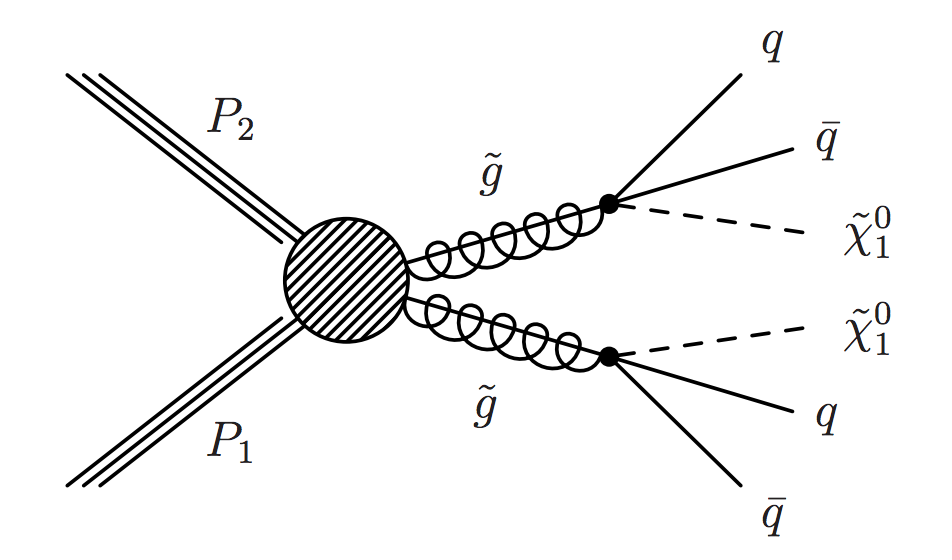
\includegraphics[width=0.4\linewidth]{T1simlifiedpp-gg-qqqqXX}\put(-32,133){(a)}
		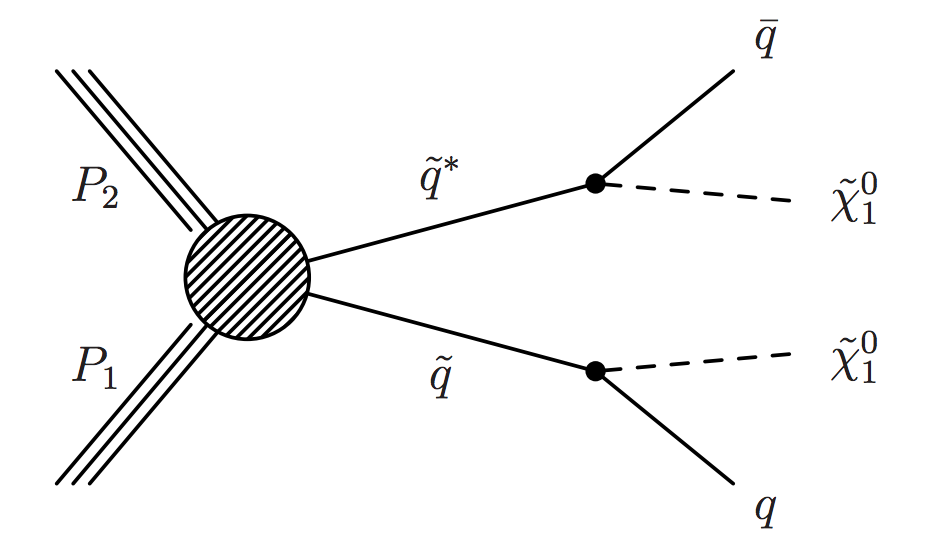
\includegraphics[width=0.4\linewidth]{T2simplifiedpp-qq-qqXX}\put(-32,133){(b)}
	\end{center}
	\caption{Simplified models of SUSY being produced at the LHC and decaying into hadrons plus missing energy \cite{MathiasSUSYthesis}}
	\label{fig:simpdecays}
\end{figure}
\\\\
The $7$ and $8$ TeV run of the LHC has not resulted in any observation of SUSY production as of yet. Instead, limits have been set on the mass of SUSY particles. It is possible that the mass of the SUSY particle has been outside of the energy range of the LHC. With the 2015 upgrade, the cross sections of such supersymmetric particles will increase by at least an order of magnitude, giving a large potential for discovery. It is also possible that the mass splitting of SUSY particles is small, known as compressed spectra. If this is the case the searches at the LHC are not as sensitive, as the energy of the jets produced in the decay to the LSP will be low. This results in a small visible component of missing energy. If SUSY exists at a scale that solves the hierarchy problem with minimal fine tuning, it should be seen at the LHC.


% the CMS bit


The Compact Muon Solenoid (CMS) detector is one of two multipurpose detectors built around proton beam collision points at the LHC. In CMS the results of collisions are measured with a series of subdetectors, built within and around a 3.8T superconducting solenoid, designed to track and record the energy of all non-neutrino SM particles \cite{CMSTechDesign1DetectorPerformance}. A representative view of CMS and its components can be seen in Fig.~\ref{fig:CMS}.
\begin{figure}
	\begin{center}
		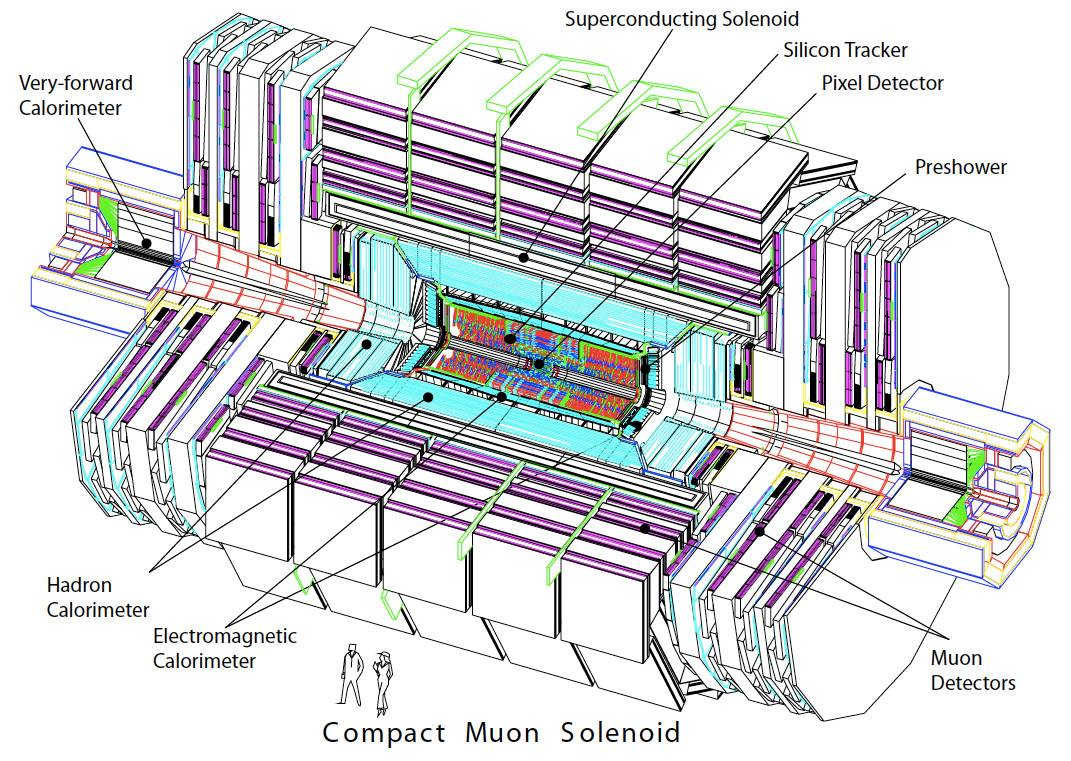
\includegraphics[width=0.8\linewidth]{cms_detector}
	\end{center}
	\caption{An internal view of the Compact Muon Solenoid detector highlighting the key detecting components \cite{CMSTechDesign1DetectorPerformance}}
	\label{fig:CMS}
\end{figure}

\subsection{The Inner Tracking System}
Within the superconducting solenoid is the silicon tracking system that can track \mbox{$p_T>1$~GeV} charged particles with an efficiency greater than $99\%$ \cite{ScienceArticle} \cite{CMSTechDesign1DetectorPerformance}. The Pixel Detector is the high granularity component of the tracking system that sits closest to the interaction point, covering the pseudorapidity region $|\eta|<2.1$ \footnote{$\eta \equiv -ln[tan\frac{\theta}{2}]$, where $\theta$ is measured with respect to the z-axis that points along the beam direction.}. The Silicon Strip Tracker sits around this with barrel and endcap components covering $|\eta|<2.4$. By measuring the curvature of their tracks, charged particle momenta can be measured with an error between $1.5\%$ and $3\%$ for $p_T\sim 100$ GeV \cite{Adam_Elwood_MSci}. The resolution of the trackers is such that the points of origin of event decay products can be inferred within $10$~$\mu$m, allowing the performance of CMS to extend up to very high pileup (number of simultaneous collisions) \cite{CMSTrackPerformance}.

\subsection{The Electromagnetic and Hadronic Calorimeters}
Surrounding the tracking system are the electromagnetic and hadronic calorimeters (ECAL and HCAL). The ECAL is constructed from 75~848 PbWO$_4$ scintillating crystals covering $|\eta|<3$. They are designed to absorb electrons and photons and emit light proportional to the energy deposited. This light is detected by custom photodiodes designed to perform well in high magnetic fields.
\\\\
The HCAL is designed to absorb hadrons and is constructed from brass absorbers interleaved with scintillating plastic tiles covering $|\eta|<3$. The scintillations are read out with hybrid photodiodes via wavelength shifting fibres.
\\\\
In the forward detector regions, the hadronic calorimetry is extended up to $|\eta|<5$ with the Forward Calorimeter, made from steel absorber with quartz scintillating fibre. To also help prevent signal contamination from low energy neutral pions there is a Preshower detector consisting of lead absorbers and silicon microstrips \cite{CMSTechDesign1DetectorPerformance}\cite{Cutajar}.

\subsection{The Muon System}
As muons are unlikely to be absorbed in the ECAL and HCAL, a muon system is built into the iron return yoke that surrounds the solenoid.  This consists of wire chambers containing ionising gas that allows the measurement of muon momenta with a greater than $1\%$ precision \cite{CMS_Overview_Chatrchyan:2008aa}.

\subsection{The Trigger and Data Acquisition System}
The rate of collisions at the LHC is so high that it would be impossible to reconstruct and store the results of all collision events. As the majority of the collisions are soft QCD processes, they are not useful in the search for new physics at the electroweak energy scale. This necessitates a multi-level trigger system that is designed to pick out and store only high centre-of-mass physics processes. The Level 1 Trigger (L1T) is the first component of the trigger system and is made from custom FPGA computational boards situated close to the detector. This uses coarse information from the calorimeters and muon system to reduce the event rate from $20$MHz (during Run 1) to $\sim100$kHz. The data from the subdetectors are then passed to the High Level Trigger (HLT), which uses full detector information to reconstruct the events and reduce the data rate to $\sim1$kHz. The remaining events are then fully reconstructed and stored at various Grid sites \cite{GridTechDesign}.


